\subsection{Part d}

By shifting the register before the addition node ``5'' to between addition node
``5'' and multiplication node ``6'', the following iteration periods are
achieved:

\begin{itemize}
	\item Loop 1:
	\begin{itemize}
		\item 4/2
	\end{itemize}
	\item Loop 2:
	\begin{itemize}
		\item 7/3
	\end{itemize}
	\item Loop 3:
	\begin{itemize}
		\item 5/2
	\end{itemize}
\end{itemize}

Therefore, the iteration period bound has been reduced.
The changes to be made can be seen in Figure \ref{fig:Q3dImg}, found below.

\begin{figure}[H]
	\centering
	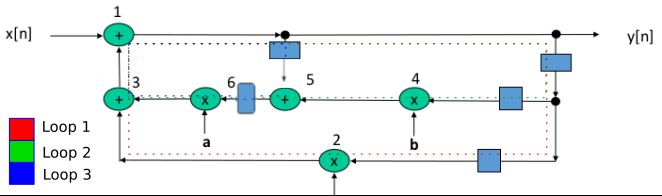
\includegraphics[width=0.8\textwidth]{images/DFGTimedLoop}
	\caption{Retimed DFG}
	\label{fig:Q3dImg}
\end{figure}
